    
    
    

    
    \hypertarget{simpsons-method-for-integration}{%
\section{Simpson's method for
integration}\label{simpsons-method-for-integration}}

    Simpson's method for integration approximates a given curve using a
number of quadratic interpolations.

The Simpson's 1/3 rule takes 3 consecutive points on the curve of the
function and represents each of those points with a quadratic function
to evaluate the area under the curve. This process is repeated for each
points, taking 3 consecutive points at a time.

\begin{figure}
\centering
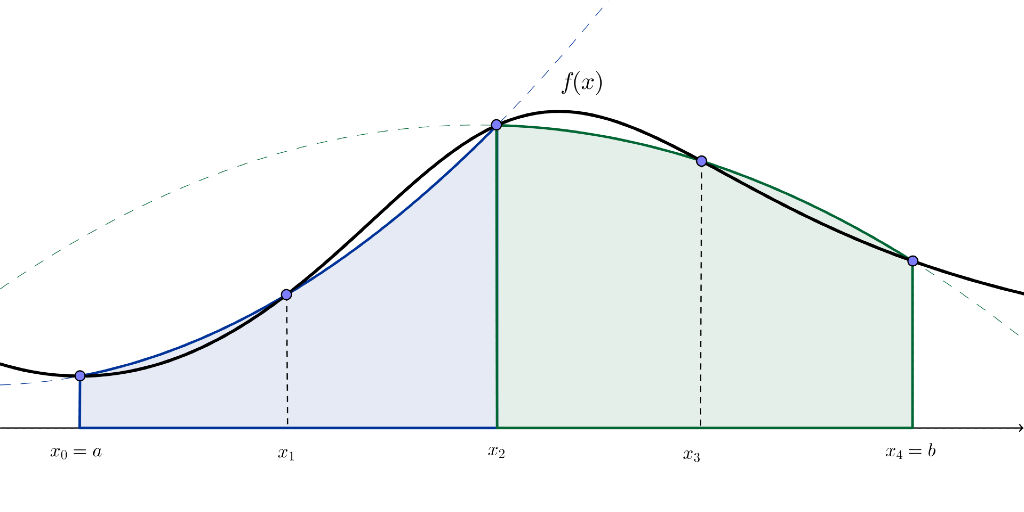
\includegraphics{resources/simpson-1.png}
\caption{resources/simpson-1.png}
\end{figure}

The result of the integration after evaluations is given by,

\[\int_a^b f(x)dx \approx \frac{h}{3} \left[ f(x_0) + 4f(x_1) + 2f(x_2) + \dots + 2f(x_{n-2}) + 4f(x_{n-1}) + f(x_n) \right]\]

    \hypertarget{code}{%
\subsection{Code}\label{code}}

    \begin{tcolorbox}[breakable, size=fbox, boxrule=1pt, pad at break*=1mm,colback=cellbackground, colframe=cellborder]
\prompt{In}{incolor}{1}{\boxspacing}
\begin{Verbatim}[commandchars=\\\{\}]
\PY{k+kn}{from} \PY{n+nn}{numpy} \PY{k+kn}{import} \PY{n}{cos}\PY{p}{,} \PY{n}{empty}\PY{p}{,} \PY{n}{pi}\PY{p}{,} \PY{n}{sin}\PY{p}{,} \PY{n}{exp}
\PY{k+kn}{from} \PY{n+nn}{matplotlib} \PY{k+kn}{import} \PY{n}{pyplot} \PY{k}{as} \PY{n}{plt}

\PY{c+c1}{\PYZsh{} Default configuaration for matplotlib}
\PY{n}{plt}\PY{o}{.}\PY{n}{style}\PY{o}{.}\PY{n}{use}\PY{p}{(}\PY{p}{[}\PY{l+s+s1}{\PYZsq{}}\PY{l+s+s1}{science}\PY{l+s+s1}{\PYZsq{}}\PY{p}{,} \PY{l+s+s1}{\PYZsq{}}\PY{l+s+s1}{ieee}\PY{l+s+s1}{\PYZsq{}}\PY{p}{]}\PY{p}{)}
\PY{n}{plt}\PY{o}{.}\PY{n}{rcParams}\PY{p}{[}\PY{l+s+s2}{\PYZdq{}}\PY{l+s+s2}{figure.figsize}\PY{l+s+s2}{\PYZdq{}}\PY{p}{]} \PY{o}{=} \PY{p}{(}\PY{l+m+mi}{10}\PY{p}{,} \PY{l+m+mi}{5}\PY{p}{)}
\end{Verbatim}
\end{tcolorbox}

    \begin{tcolorbox}[breakable, size=fbox, boxrule=1pt, pad at break*=1mm,colback=cellbackground, colframe=cellborder]
\prompt{In}{incolor}{2}{\boxspacing}
\begin{Verbatim}[commandchars=\\\{\}]
\PY{c+c1}{\PYZsh{} Function to generate `n` evenly spaced points between limits `a` and `b`}
\PY{k}{def} \PY{n+nf}{generate\PYZus{}points}\PY{p}{(}\PY{n}{a}\PY{p}{,} \PY{n}{b}\PY{p}{,} \PY{n}{n}\PY{p}{,} \PY{n}{retstep}\PY{o}{=}\PY{k+kc}{False}\PY{p}{)}\PY{p}{:}

    \PY{c+c1}{\PYZsh{} Calculating the spacing (difference) between each points}
    \PY{n}{h} \PY{o}{=} \PY{p}{(}\PY{n}{b} \PY{o}{\PYZhy{}} \PY{n}{a}\PY{p}{)} \PY{o}{/} \PY{p}{(}\PY{n}{n} \PY{o}{\PYZhy{}} \PY{l+m+mi}{1}\PY{p}{)}

    \PY{c+c1}{\PYZsh{} Creating an empty array to store the points}
    \PY{n}{points} \PY{o}{=} \PY{n}{empty}\PY{p}{(}\PY{n}{n}\PY{p}{)}

    \PY{c+c1}{\PYZsh{} Generating the points}
    \PY{k}{for} \PY{n}{i} \PY{o+ow}{in} \PY{n+nb}{range}\PY{p}{(}\PY{n}{n}\PY{p}{)}\PY{p}{:}
        \PY{n}{points}\PY{p}{[}\PY{n}{i}\PY{p}{]} \PY{o}{=} \PY{n}{a}
        \PY{n}{a} \PY{o}{+}\PY{o}{=} \PY{n}{h}

    \PY{c+c1}{\PYZsh{} Returning the difference between each points if asked for}
    \PY{k}{if} \PY{n}{retstep}\PY{p}{:}
        \PY{k}{return} \PY{n}{points}\PY{p}{,} \PY{n}{h}

    \PY{k}{return} \PY{n}{points}
\end{Verbatim}
\end{tcolorbox}

    \begin{tcolorbox}[breakable, size=fbox, boxrule=1pt, pad at break*=1mm,colback=cellbackground, colframe=cellborder]
\prompt{In}{incolor}{3}{\boxspacing}
\begin{Verbatim}[commandchars=\\\{\}]
\PY{c+c1}{\PYZsh{} Importing code for Simpson\PYZsq{}s method for integration}
\PY{k}{def} \PY{n+nf}{integrate\PYZus{}simpson}\PY{p}{(}\PY{n}{f}\PY{p}{,} \PY{n}{a}\PY{p}{,} \PY{n}{b}\PY{p}{,} \PY{n}{n}\PY{p}{)}\PY{p}{:}

    \PY{c+c1}{\PYZsh{} Checking if interation using Simpson\PYZsq{}s method is possible}
    \PY{k}{if} \PY{n}{n} \PY{o}{\PYZpc{}} \PY{l+m+mi}{2} \PY{o}{==} \PY{l+m+mi}{0} \PY{o+ow}{or} \PY{n}{n} \PY{o}{\PYZlt{}} \PY{l+m+mi}{2}\PY{p}{:}
        \PY{k}{raise} \PY{n+ne}{ValueError}\PY{p}{(}
            \PY{l+s+s2}{\PYZdq{}}\PY{l+s+s2}{Intergration using Simpson}\PY{l+s+s2}{\PYZsq{}}\PY{l+s+s2}{s method can only be evaluated for odd number of points greater than 2!}\PY{l+s+s2}{\PYZdq{}}\PY{p}{)}

    \PY{c+c1}{\PYZsh{} Generating points}
    \PY{n}{x}\PY{p}{,} \PY{n}{h} \PY{o}{=} \PY{n}{generate\PYZus{}points}\PY{p}{(}\PY{n}{a}\PY{p}{,} \PY{n}{b}\PY{p}{,} \PY{n}{n}\PY{p}{,} \PY{n}{retstep}\PY{o}{=}\PY{k+kc}{True}\PY{p}{)}

    \PY{c+c1}{\PYZsh{} Evaluating the function `f(x)` for each points}
    \PY{n}{y} \PY{o}{=} \PY{n}{f}\PY{p}{(}\PY{n}{x}\PY{p}{)}

    \PY{c+c1}{\PYZsh{} Declaring a variable to store the integral}
    \PY{n}{integral} \PY{o}{=} \PY{l+m+mi}{0}

    \PY{c+c1}{\PYZsh{} Evaluating the integral using Simpson\PYZsq{}s method}
    \PY{k}{for} \PY{n}{i} \PY{o+ow}{in} \PY{n+nb}{range}\PY{p}{(}\PY{n}{n}\PY{p}{)}\PY{p}{:}
        \PY{k}{if} \PY{n}{i} \PY{o}{==} \PY{l+m+mi}{0} \PY{o+ow}{or} \PY{n}{i} \PY{o}{==} \PY{p}{(}\PY{n}{n} \PY{o}{\PYZhy{}} \PY{l+m+mi}{1}\PY{p}{)}\PY{p}{:}
            \PY{n}{integral} \PY{o}{+}\PY{o}{=} \PY{n}{y}\PY{p}{[}\PY{n}{i}\PY{p}{]}
        \PY{k}{elif} \PY{n}{i} \PY{o}{\PYZpc{}} \PY{l+m+mi}{2} \PY{o}{==} \PY{l+m+mi}{0}\PY{p}{:}
            \PY{n}{integral} \PY{o}{+}\PY{o}{=} \PY{n}{y}\PY{p}{[}\PY{n}{i}\PY{p}{]} \PY{o}{*} \PY{l+m+mi}{2}
        \PY{k}{elif} \PY{n}{i} \PY{o}{\PYZpc{}} \PY{l+m+mi}{2} \PY{o}{==} \PY{l+m+mi}{1}\PY{p}{:}
            \PY{n}{integral} \PY{o}{+}\PY{o}{=} \PY{n}{y}\PY{p}{[}\PY{n}{i}\PY{p}{]} \PY{o}{*} \PY{l+m+mi}{4}

    \PY{n}{integral} \PY{o}{*}\PY{o}{=} \PY{p}{(}\PY{n}{h} \PY{o}{/} \PY{l+m+mi}{3}\PY{p}{)}

    \PY{k}{return} \PY{n}{integral}
\end{Verbatim}
\end{tcolorbox}

    \hypertarget{examples}{%
\subsection{Examples}\label{examples}}

    \hypertarget{int_02pi-sinx-cdot-dx}{%
\subsubsection{\texorpdfstring{\[\int_{0}^{2\pi} sin(x) \cdot dx\]}{\textbackslash int\_\{0\}\^{}\{2\textbackslash pi\} sin(x) \textbackslash cdot dx}}\label{int_02pi-sinx-cdot-dx}}

    \begin{tcolorbox}[breakable, size=fbox, boxrule=1pt, pad at break*=1mm,colback=cellbackground, colframe=cellborder]
\prompt{In}{incolor}{4}{\boxspacing}
\begin{Verbatim}[commandchars=\\\{\}]
\PY{k}{def} \PY{n+nf}{f}\PY{p}{(}\PY{n}{x}\PY{p}{)}\PY{p}{:}
    \PY{k}{return} \PY{n}{sin}\PY{p}{(}\PY{n}{x}\PY{p}{)}


\PY{n}{x\PYZus{}i} \PY{o}{=} \PY{l+m+mi}{0}
\PY{n}{x\PYZus{}f} \PY{o}{=} \PY{l+m+mi}{2} \PY{o}{*} \PY{n}{pi}
\PY{n}{n} \PY{o}{=} \PY{l+m+mi}{1001}
\end{Verbatim}
\end{tcolorbox}

    \begin{tcolorbox}[breakable, size=fbox, boxrule=1pt, pad at break*=1mm,colback=cellbackground, colframe=cellborder]
\prompt{In}{incolor}{5}{\boxspacing}
\begin{Verbatim}[commandchars=\\\{\}]
\PY{n}{x} \PY{o}{=} \PY{n}{generate\PYZus{}points}\PY{p}{(}\PY{n}{x\PYZus{}i}\PY{p}{,} \PY{n}{x\PYZus{}f}\PY{p}{,} \PY{n}{n}\PY{p}{)}
\PY{n}{plt}\PY{o}{.}\PY{n}{plot}\PY{p}{(}\PY{n}{x}\PY{p}{,} \PY{n}{f}\PY{p}{(}\PY{n}{x}\PY{p}{)}\PY{p}{,} \PY{n}{label}\PY{o}{=}\PY{l+s+s2}{\PYZdq{}}\PY{l+s+s2}{\PYZdl{}sin(x)\PYZdl{}}\PY{l+s+s2}{\PYZdq{}}\PY{p}{)}
\PY{n}{plt}\PY{o}{.}\PY{n}{legend}\PY{p}{(}\PY{p}{)}
\PY{n}{plt}\PY{o}{.}\PY{n}{show}\PY{p}{(}\PY{p}{)}
\end{Verbatim}
\end{tcolorbox}

    \begin{center}
    \adjustimage{max size={0.9\linewidth}{0.9\paperheight}}{4_Simpsons_method_for_integration_files/4_Simpsons_method_for_integration_9_0.png}
    \end{center}
    { \hspace*{\fill} \\}
    
    \begin{tcolorbox}[breakable, size=fbox, boxrule=1pt, pad at break*=1mm,colback=cellbackground, colframe=cellborder]
\prompt{In}{incolor}{6}{\boxspacing}
\begin{Verbatim}[commandchars=\\\{\}]
\PY{n}{integrate\PYZus{}simpson}\PY{p}{(}\PY{n}{f}\PY{p}{,} \PY{n}{x\PYZus{}i}\PY{p}{,} \PY{n}{x\PYZus{}f}\PY{p}{,} \PY{n}{n}\PY{p}{)}
\end{Verbatim}
\end{tcolorbox}

            \begin{tcolorbox}[breakable, size=fbox, boxrule=.5pt, pad at break*=1mm, opacityfill=0]
\prompt{Out}{outcolor}{6}{\boxspacing}
\begin{Verbatim}[commandchars=\\\{\}]
-1.1860553938477683e-13
\end{Verbatim}
\end{tcolorbox}
        
    \hypertarget{int_-pipi-e-x2-cdot-dx}{%
\subsubsection{\texorpdfstring{\[\int_{-\pi}^{\pi} e^{-x^2} \cdot dx\]}{\textbackslash int\_\{-\textbackslash pi\}\^{}\{\textbackslash pi\} e\^{}\{-x\^{}2\} \textbackslash cdot dx}}\label{int_-pipi-e-x2-cdot-dx}}

    \begin{tcolorbox}[breakable, size=fbox, boxrule=1pt, pad at break*=1mm,colback=cellbackground, colframe=cellborder]
\prompt{In}{incolor}{7}{\boxspacing}
\begin{Verbatim}[commandchars=\\\{\}]
\PY{k}{def} \PY{n+nf}{f}\PY{p}{(}\PY{n}{x}\PY{p}{)}\PY{p}{:}
    \PY{k}{return} \PY{n}{exp}\PY{p}{(}\PY{o}{\PYZhy{}}\PY{p}{(}\PY{n}{x}\PY{o}{*}\PY{o}{*}\PY{l+m+mi}{2}\PY{p}{)}\PY{p}{)}


\PY{n}{x\PYZus{}i} \PY{o}{=} \PY{o}{\PYZhy{}} \PY{n}{pi}
\PY{n}{x\PYZus{}f} \PY{o}{=} \PY{n}{pi}
\PY{n}{n} \PY{o}{=} \PY{l+m+mi}{1001}
\end{Verbatim}
\end{tcolorbox}

    \begin{tcolorbox}[breakable, size=fbox, boxrule=1pt, pad at break*=1mm,colback=cellbackground, colframe=cellborder]
\prompt{In}{incolor}{8}{\boxspacing}
\begin{Verbatim}[commandchars=\\\{\}]
\PY{n}{x} \PY{o}{=} \PY{n}{generate\PYZus{}points}\PY{p}{(}\PY{n}{x\PYZus{}i}\PY{p}{,} \PY{n}{x\PYZus{}f}\PY{p}{,} \PY{n}{n}\PY{p}{)}
\PY{n}{plt}\PY{o}{.}\PY{n}{plot}\PY{p}{(}\PY{n}{x}\PY{p}{,} \PY{n}{f}\PY{p}{(}\PY{n}{x}\PY{p}{)}\PY{p}{,} \PY{n}{label}\PY{o}{=}\PY{l+s+s2}{\PYZdq{}}\PY{l+s+s2}{\PYZdl{}e\PYZca{}}\PY{l+s+s2}{\PYZob{}}\PY{l+s+s2}{\PYZhy{}x\PYZca{}2\PYZcb{}\PYZdl{}}\PY{l+s+s2}{\PYZdq{}}\PY{p}{)}
\PY{n}{plt}\PY{o}{.}\PY{n}{legend}\PY{p}{(}\PY{p}{)}
\PY{n}{plt}\PY{o}{.}\PY{n}{show}\PY{p}{(}\PY{p}{)}
\end{Verbatim}
\end{tcolorbox}

    \begin{center}
    \adjustimage{max size={0.9\linewidth}{0.9\paperheight}}{4_Simpsons_method_for_integration_files/4_Simpsons_method_for_integration_13_0.png}
    \end{center}
    { \hspace*{\fill} \\}
    
    \begin{tcolorbox}[breakable, size=fbox, boxrule=1pt, pad at break*=1mm,colback=cellbackground, colframe=cellborder]
\prompt{In}{incolor}{9}{\boxspacing}
\begin{Verbatim}[commandchars=\\\{\}]
\PY{n}{integrate\PYZus{}simpson}\PY{p}{(}\PY{n}{f}\PY{p}{,} \PY{n}{x\PYZus{}i}\PY{p}{,} \PY{n}{x\PYZus{}f}\PY{p}{,} \PY{n}{n}\PY{p}{)}
\end{Verbatim}
\end{tcolorbox}

            \begin{tcolorbox}[breakable, size=fbox, boxrule=.5pt, pad at break*=1mm, opacityfill=0]
\prompt{Out}{outcolor}{9}{\boxspacing}
\begin{Verbatim}[commandchars=\\\{\}]
1.7724381183455118
\end{Verbatim}
\end{tcolorbox}
        
    \hypertarget{int_fraca-pibfracapib-e-a-bx2-cdot-dx}{%
\subsubsection{\texorpdfstring{\[\int_{\frac{a-\pi}{b}}^{\frac{a+\pi}{b}} e^{-(a-bx)^2} \cdot dx\]}{\textbackslash int\_\{\textbackslash frac\{a-\textbackslash pi\}\{b\}\}\^{}\{\textbackslash frac\{a+\textbackslash pi\}\{b\}\} e\^{}\{-(a-bx)\^{}2\} \textbackslash cdot dx}}\label{int_fraca-pibfracapib-e-a-bx2-cdot-dx}}

for, \[a = 1000, \; b = 0.1\]

    \begin{tcolorbox}[breakable, size=fbox, boxrule=1pt, pad at break*=1mm,colback=cellbackground, colframe=cellborder]
\prompt{In}{incolor}{10}{\boxspacing}
\begin{Verbatim}[commandchars=\\\{\}]
\PY{n}{a} \PY{o}{=} \PY{l+m+mi}{1000}
\PY{n}{b} \PY{o}{=} \PY{l+m+mf}{0.5}


\PY{k}{def} \PY{n+nf}{f}\PY{p}{(}\PY{n}{x}\PY{p}{,} \PY{n}{a}\PY{o}{=}\PY{n}{a}\PY{p}{,} \PY{n}{b}\PY{o}{=}\PY{n}{b}\PY{p}{)}\PY{p}{:}
    \PY{k}{return} \PY{n}{exp}\PY{p}{(}\PY{o}{\PYZhy{}}\PY{p}{(}\PY{p}{(}\PY{n}{a} \PY{o}{\PYZhy{}} \PY{n}{b} \PY{o}{*} \PY{n}{x}\PY{p}{)}\PY{o}{*}\PY{o}{*}\PY{l+m+mi}{2}\PY{p}{)}\PY{p}{)}


\PY{n}{x\PYZus{}i} \PY{o}{=} \PY{p}{(}\PY{n}{a} \PY{o}{\PYZhy{}} \PY{n}{pi}\PY{p}{)} \PY{o}{/} \PY{n}{b}
\PY{n}{x\PYZus{}f} \PY{o}{=} \PY{p}{(}\PY{n}{a} \PY{o}{+} \PY{n}{pi}\PY{p}{)} \PY{o}{/} \PY{n}{b}
\PY{n}{n} \PY{o}{=} \PY{l+m+mi}{1001}
\end{Verbatim}
\end{tcolorbox}

    \begin{tcolorbox}[breakable, size=fbox, boxrule=1pt, pad at break*=1mm,colback=cellbackground, colframe=cellborder]
\prompt{In}{incolor}{11}{\boxspacing}
\begin{Verbatim}[commandchars=\\\{\}]
\PY{n}{x} \PY{o}{=} \PY{n}{generate\PYZus{}points}\PY{p}{(}\PY{n}{x\PYZus{}i}\PY{p}{,} \PY{n}{x\PYZus{}f}\PY{p}{,} \PY{n}{n}\PY{p}{)}
\PY{n}{plt}\PY{o}{.}\PY{n}{plot}\PY{p}{(}\PY{n}{x}\PY{p}{,} \PY{n}{f}\PY{p}{(}\PY{n}{x}\PY{p}{)}\PY{p}{,} \PY{n}{label}\PY{o}{=}\PY{l+s+s2}{\PYZdq{}}\PY{l+s+s2}{\PYZdl{}e\PYZca{}}\PY{l+s+s2}{\PYZob{}}\PY{l+s+s2}{\PYZhy{}(a\PYZhy{}bx)\PYZca{}2\PYZcb{}\PYZdl{}}\PY{l+s+s2}{\PYZdq{}}\PY{p}{)}
\PY{n}{plt}\PY{o}{.}\PY{n}{legend}\PY{p}{(}\PY{p}{)}
\PY{n}{plt}\PY{o}{.}\PY{n}{show}\PY{p}{(}\PY{p}{)}
\end{Verbatim}
\end{tcolorbox}

    \begin{center}
    \adjustimage{max size={0.9\linewidth}{0.9\paperheight}}{4_Simpsons_method_for_integration_files/4_Simpsons_method_for_integration_17_0.png}
    \end{center}
    { \hspace*{\fill} \\}
    
    \begin{tcolorbox}[breakable, size=fbox, boxrule=1pt, pad at break*=1mm,colback=cellbackground, colframe=cellborder]
\prompt{In}{incolor}{12}{\boxspacing}
\begin{Verbatim}[commandchars=\\\{\}]
\PY{n}{integrate\PYZus{}simpson}\PY{p}{(}\PY{n}{f}\PY{p}{,} \PY{n}{x\PYZus{}i}\PY{p}{,} \PY{n}{x\PYZus{}f}\PY{p}{,} \PY{n}{n}\PY{p}{)}
\end{Verbatim}
\end{tcolorbox}

            \begin{tcolorbox}[breakable, size=fbox, boxrule=.5pt, pad at break*=1mm, opacityfill=0]
\prompt{Out}{outcolor}{12}{\boxspacing}
\begin{Verbatim}[commandchars=\\\{\}]
3.544876236673206
\end{Verbatim}
\end{tcolorbox}
        
    \hypertarget{int_-pipi-x2-e-x2-cdot-dx}{%
\subsubsection{\texorpdfstring{\[\int_{-\pi}^{\pi} x^2 e^{-x^2} \cdot dx\]}{\textbackslash int\_\{-\textbackslash pi\}\^{}\{\textbackslash pi\} x\^{}2 e\^{}\{-x\^{}2\} \textbackslash cdot dx}}\label{int_-pipi-x2-e-x2-cdot-dx}}

    \begin{tcolorbox}[breakable, size=fbox, boxrule=1pt, pad at break*=1mm,colback=cellbackground, colframe=cellborder]
\prompt{In}{incolor}{13}{\boxspacing}
\begin{Verbatim}[commandchars=\\\{\}]
\PY{k}{def} \PY{n+nf}{f}\PY{p}{(}\PY{n}{x}\PY{p}{)}\PY{p}{:}
    \PY{k}{return} \PY{n}{x}\PY{o}{*}\PY{o}{*}\PY{l+m+mi}{2} \PY{o}{*} \PY{n}{exp}\PY{p}{(}\PY{o}{\PYZhy{}}\PY{n}{x}\PY{o}{*}\PY{o}{*}\PY{l+m+mi}{2}\PY{p}{)}


\PY{n}{x\PYZus{}i} \PY{o}{=} \PY{o}{\PYZhy{}} \PY{n}{pi}
\PY{n}{x\PYZus{}f} \PY{o}{=} \PY{n}{pi}
\PY{n}{n} \PY{o}{=} \PY{l+m+mi}{1001}
\end{Verbatim}
\end{tcolorbox}

    \begin{tcolorbox}[breakable, size=fbox, boxrule=1pt, pad at break*=1mm,colback=cellbackground, colframe=cellborder]
\prompt{In}{incolor}{14}{\boxspacing}
\begin{Verbatim}[commandchars=\\\{\}]
\PY{n}{x} \PY{o}{=} \PY{n}{generate\PYZus{}points}\PY{p}{(}\PY{n}{x\PYZus{}i}\PY{p}{,} \PY{n}{x\PYZus{}f}\PY{p}{,} \PY{n}{n}\PY{p}{)}
\PY{n}{plt}\PY{o}{.}\PY{n}{plot}\PY{p}{(}\PY{n}{x}\PY{p}{,} \PY{n}{f}\PY{p}{(}\PY{n}{x}\PY{p}{)}\PY{p}{,} \PY{n}{label}\PY{o}{=}\PY{l+s+s2}{\PYZdq{}}\PY{l+s+s2}{\PYZdl{}x\PYZca{}2e\PYZca{}}\PY{l+s+s2}{\PYZob{}}\PY{l+s+s2}{\PYZhy{}x\PYZca{}2\PYZcb{}\PYZdl{}}\PY{l+s+s2}{\PYZdq{}}\PY{p}{)}
\PY{n}{plt}\PY{o}{.}\PY{n}{legend}\PY{p}{(}\PY{p}{)}
\PY{n}{plt}\PY{o}{.}\PY{n}{show}\PY{p}{(}\PY{p}{)}
\end{Verbatim}
\end{tcolorbox}

    \begin{center}
    \adjustimage{max size={0.9\linewidth}{0.9\paperheight}}{4_Simpsons_method_for_integration_files/4_Simpsons_method_for_integration_21_0.png}
    \end{center}
    { \hspace*{\fill} \\}
    
    \begin{tcolorbox}[breakable, size=fbox, boxrule=1pt, pad at break*=1mm,colback=cellbackground, colframe=cellborder]
\prompt{In}{incolor}{15}{\boxspacing}
\begin{Verbatim}[commandchars=\\\{\}]
\PY{n}{integrate\PYZus{}simpson}\PY{p}{(}\PY{n}{f}\PY{p}{,} \PY{n}{x\PYZus{}i}\PY{p}{,} \PY{n}{x\PYZus{}f}\PY{p}{,} \PY{n}{n}\PY{p}{)}
\end{Verbatim}
\end{tcolorbox}

            \begin{tcolorbox}[breakable, size=fbox, boxrule=.5pt, pad at break*=1mm, opacityfill=0]
\prompt{Out}{outcolor}{15}{\boxspacing}
\begin{Verbatim}[commandchars=\\\{\}]
0.8860565659897861
\end{Verbatim}
\end{tcolorbox}
        

    % Add a bibliography block to the postdoc
    
    
    
